\documentclass{article}
\usepackage[T1]{fontenc}
\usepackage{lmodern}
\usepackage{graphicx}
\usepackage{amsmath,amssymb}
\usepackage[a4paper,margin=2cm]{geometry}
\usepackage[absolute,overlay]{textpos}
\setlength{\TPHorizModule}{1mm}
\setlength{\TPVertModule}{1mm}
\usepackage[indonesian]{babel}
\usepackage{hyperref}
\setlength{\emergencystretch}{2em}
% unit: Halaman 13

\begin{document}

% === Halaman 13 (python/native) ===

3. Yakin pengirim pesan adalah 

asli (authentication), bukan 

pihak ketiga yang menyerupai.

13

4. Pengirim pesan tidak dapat 

menyangkal (non repudiation) telah 

mengirim pesan.

Dia mengklaim bahwa dia adalah A

A

B

% deskripsi: gambar native xref 76
\noindent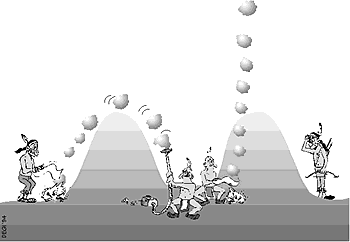
\includegraphics[width=0.85\textwidth]{../../images/python/page_013_img_01.png}

% deskripsi: gambar native xref 77
\noindent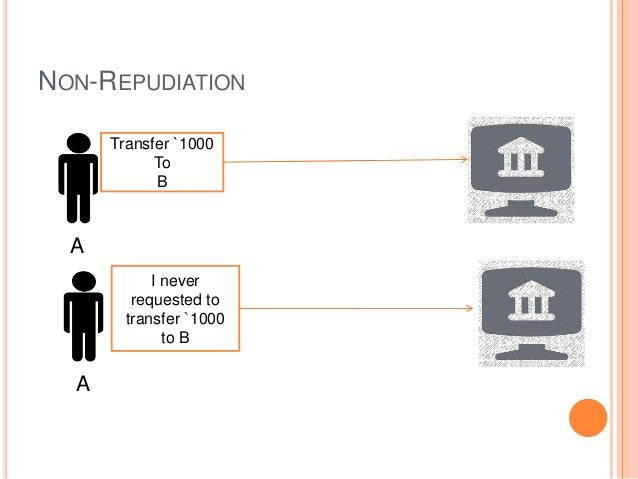
\includegraphics[width=0.85\textwidth]{../../images/python/page_013_img_02.jpeg}

\end{document}
